\documentclass[11pt]{article}
\usepackage{hyperref}
\usepackage{common}
\title{HW4 All About Attention}
\author{Roshan Padaki \\ rpadaki@college.harvard.edu \and Michael Zhang \\ michael\_zhang@college.harvard.edu }
\begin{document}

\maketitle{}
\section{Introduction}

Natural language inference (NLI) is a central problem in NLP, where given two input sentences denoted the premise and the hypothesis, we would like to determine whether the hypothesis supports and entails the premise, or contradicts it. Towards this, \citep{DBLP:journals/corr/ParikhT0U16} introduce a new model for NLI, deviating from the zeitgeist at the time of convolutional networks (CNNs) or long short-term memory networks (LSTMs). Instead they claim that it is enough to simply align bits of local text substructure for the task, intuitively learning to pay attention to similar parts of premise-hypothesis pairs that matter. 

In this assignment, we aim to recreate their presented decomposable attention model, both in its vanilla implementation and an extended intra-attention variant. Additionally, we explore two ensembling extensions. First we implement a mixture of models with a uniform prior, training with exact log marginal likelihood. We next consider training the mixture of models with a VAE, describing the methods and results.  

\section{Problem Description}
We define the task of NLI as according to \citep{DBLP:journals/corr/ParikhT0U16}. Let $\mathbf{a} = (a_1, \ldots , a_{l_{a}})$ and $\mathbf{b} = (a_1, \ldots, a_{1_{b}})$ be two input sentences of length $l_a$ and $l_b$ respectively. Furthermore, in these pairings we refer to $\mathbf{a}$ as the premise and $\mathbf{b}$ as the hypothesis. We assume that each $a_i, b_j \in \mathbb{R}^d$ is a word embedding vector of dimension $d$, which may come from the standard output of feeding the sentences in their observed forms into a pretrained embedding model such as Word2Vec or GLoVE \citep{Pennington14glove:global}. Our training data comes in the form of labeled tuples
$
\{ \mathbf{a}^{(n)}, \mathbf{b}^{(n)}, \mathbf{y}^{(n)}\}^N_{n=1}
$
where $\mathbf{y}^{n} = (y_1^(n), \ldots y_C^{(n)}$ is an indicator vector encoding the label and $C$ is the number of output classes. Accordingly, at test time we would like to predict the correct label $\mathbf{y}$ given a pair of input sentences $(\mathbf{a}, \mathbf{b})$.



% \begin{center}
%     \begin{tabular}{@{}lll@{}}
%         % \toprule
%         &\multicolumn{2}{c}{} \\
%         & Variable & Definition\\
%         \midrule
%         & $\sigma$ & Activation function (sigmoid, tanh, ReLU) \\
%         & $\boldb$ & Bias term(s) \\
%         & $\bolde$ & Embedding vector \\
%         & $\boldx$ & Word vector \\
%         & $\boldw, p, c$ & Convolutional terms: filter, dropout prob., feature\\
%         & $\mcP, \mcN$ & Training data: positive sentences, negative sentences \\
%         \bottomrule
%     \end{tabular}
% \end{center}


\section{Model and Algorithms}
As mentioned earlier, we implemented and trained four models: a vanilla decomposable attention network, the former with intra-attention, a mixture of models ensembling multiple decomposable networks trained with exact marginal log-likelihood, and a mixture of models trained with a VAE. We further describe these models below.

\subsection{Vanilla Decomposable Attention Model}
Our vanilla attention model comprises of deep neural net capable of end-to-end training over the tasks of input representation, attention, sentence comparison, and aggregation as described in \citep{DBLP:journals/corr/ParikhT0U16}. In this version, we are given input representations $\bar{\mathbf{a}} = (\bar{a}_1, \ldots, \bar{a}_{l_a})$ and $\bar{\mathbf{b}} = (\bar{b}_1, \ldots, \bar{b}_{l_b})$ of our sentences, which are directly fed into the rest of the model. We note that this does not make use of word ordering, and describe the relevant modifications using some sequence information in the intra-attention section. To train, we first soft-align elements of $\bar{\mathbf{a}}$ and $\bar{\mathbf{b}}$, compare the aligned subphrases to produce a set of nonlinear combinations of $a_i$ and its softly-aligned counterpart in $\mathbf{b}$ for all $i$, and finally aggregate the sets to predict a label $\hat{y}$. We describe these core components more in depth as follows:

\subsubsection{Attention}
We first use a standard feed-forward neural network with ReLU activation $F$ and input $(\bar{a}_i, \bar{b}_i)$ to produce unnormalized attention weights $e_{ij}$ such that 
\[
e_{ij} := F'(\bar{a}_i, \bar{b}_j) = F(\bar{a}_i)^T F(\bar{b}_j)
\]
and achieve the subphrases $\beta_i$ and $\alpha_j$ softly-aligned to $\bar{a}_i$ and $\bar{b}_j$ respectively by normalizing such that
\[
\beta_i := \sum_{j=1}^l_b \frac{\exp(e_{ij})}{\sum_{k=1}^{l_b} \exp(e_{ik})} \bar{b}_j
\text{ and }
\alpha_i := \sum_{i=1}^l_a \frac{\exp(e_{ij})}{\sum_{k=1}^{l_a} \exp(e_{ik})} \bar{a}_j
\]

\subsubsection{Comparison}
Following this, we compare the aligned phrases by using concatenated pairs as inputs into another feed-forward network $G$, concatenating the aligned pairs. Accordingly, for all $i \in [1, \ldots, l_a]$ and $j \in [1, \ldots, 1_b]$, we end up with comparison vectors
\[
\textbf{v}_{1,i} := G([\bar{a}_i, \beta_i]) \text{ and } \textbf{v}_{2,i} := G([\bar{b}_i, \alpha_i])
\]
where $[\cdot, \cdot]$ denotes concatenation between the two inputs.

\subsubsection{Aggregation}
The last step involves yet another neural net $H$, which classifies our comparison outputs to predict a class $\hat{y}$. To do so, given two sets of comparison vectors $\{\mathbf{v}_{1, i}\}_{i=1}^{l_a}$ and $\{\mathbf{v}_{2, i}\}_{i=1}^{l_b}$, we take their sums
\[
\mathbf{v}_1 = \sum_{i=1}^{l_a}\mathbf{v}_{1, i} 
\text{ and }
\mathbf{v}_2 = \sum_{i=1}^{l_b}\mathbf{v}_{2, i}
\]
and get a vector of scores $\hat{\mathbf{y}} = H([\mathbf{v}_1, \mathbf{v}_2]) \in \mathbb{R}^C$ where $C$ is the number of label classes. We then pick the label with the highest score, i.e. for the $i$-th sentence input, $\hat{y}_i = \arg \max_i \hat{\mathbf{y}}_i$.
Our models train with multi-class cross-entropy loss with dropout regularization, such that with learnable parameters $\theta_F, \theta_G, \theta_H$ for neural nets $F, G, H$ respectively, we optimize against the loss
\[
L(\theta_F, \theta_G, \theta_H) = \frac{1}{N}\sum_{n=1}^N \sum_{c=1}^C y_c^{(n)}\log \frac{\exp (\hat{y}_c)}{\sum_{c' = 1}^C \exp (\hat{y}_c')}
\]

\subsection{Intra-Attention}
As a direct follow-up to the previous model, we augment the input representation with intra-sentence attention or intra-attention to incoporate some sequential information about the words within each sentence. Using distance-sensitive bias terms $d_{i-j} \in \mathbb{R}$, we then train intra-attention variants of $F$ similar to the above such that
\[
f_{ij} := F_{\text{intra}}(a_i)^T F_{\text{intra}}(a_j)
\]
which leads to self-aligned phrases
\[
a_{i} := \sum_{j=1}^{l_a} \frac{\exp(f_{ij} + d_{i-j}}{\sum_{k=1}^{l_a} \exp(f_{ik} + d_{i-k)}} a_j
% \text{ and }
% \alpha_i := \sum_{i=1}^l_a \frac{\exp(e_{ij})}{\sum_{k=1}^{l_a} \exp(e_{ik})} \bar{a}_j
\]

\subsection{Mixture of Models}
Beyond the single model setups, we also train with multiple models, using latent variables as a form of ensembling. Accordingly, with the same objective of outputting likelihoods $p(y | \mathbf{a}, \mathbf{b}; \theta)$ where $\theta = (\theta_F, \theta_G, \theta_H)$, we use $K$ models $p(y | \mathbf{a}, \mathbf{b}; \theta_k)$. In our vanilla setup, we use a discrete latent variable $c \in \text{Unif}(1, \ldots K)$ to determine which model is being used to produce our prediction $\hat{y}$, and obtain marginal likelihood over all models 
\[
p(y| \mathbf{a}, \mathbf{b}; \theta) = \sum_{c=1}^K p(c) p(y | \mathbf{a}, \mathbf{b}; \theta_c)
\]
In our experiments, $K$ is small, so we can enumerate over all $c$. Given our prior, this is akin to empirically taking the average over the set of our defined models.

\subsection{Mixture of Models with VAE Training}
Finally we explore training with a Variational Auto-Encoder (VAE) to perform efficient training. Given inference network $q(c | y, \mathbf{a}, \mathbf{b})$ we get the evidence (ELBO)
\[
\log p(y | \mathbf{a}, \mathbf{b} \; \theta) \geq \mathbb{E}_{c \sim q(c | y, \mathbf{a}, \mathbf{b})} \log p(y \mid \mathbf{a}, \mathbf{b}\; \theta_c) - \text{KL}(q(c \mid y, \mathbf{a}, \mathbf{b}) || p(c))
\]
where $\text{KL}$ is the KL-divergence and $p(c)$ is our prior. Towards being able to differentiate the expectation, we use REINFORCE \citep{NIPS1999_1713} to estimate the gradients such that
\[
\nabla \mathbb{E}_{c \sim q(c | y \mathbf{a}, \mathbf{b})} \log p(y \mid \mathbf{a}, \mathbf{b}; \theta_c) = \mathbb{E}_{c \sim q(c | y \mathbf{a}, \mathbf{b})} \left[ \nabla \log p(y \mid \mathbf{a}, \mathbf{b} \theta_c) + \log p(y \mid \mathbf{a}, \mathbf{b} \; \theta_c) \nabla \log q(c \mid y, \mathbf{a}, \mathbf{b}) \right]
\]

% Here you specify the model itself. This section should formally
% describe the model used to solve the task proposed in the previous
% section. This section should try to avoid introducing new vocabulary
% or notation, when possible use the notation from the previous section.
% Feel free to use the notation from class, but try to make the note
% understandable as a standalone piece of text.

% This section is also a great place to include other material that
% describes the underlying structure and choices of your model, for
% instance here are some example tables and algorithms from full
% research papers:

% \begin{itemize}
% \item diagrams of your model,

%   \begin{center}
%     \includegraphics[width=0.4\textwidth]{network}
%   \end{center}
% \item feature tables,

%   \begin{center}
%     \begin{tabular}{@{}lll@{}}
%       \toprule
%       &\multicolumn{2}{c}{Mention Features  } \\
%       & Feature & Value Set\\
%       \midrule
%       & Mention Head & $\mcV$ \\
%       & Mention First Word & $\mcV$ \\
%       & Mention Last Word & $\mcV$ \\
%       & Word Preceding Mention & $\mcV$ \\
%       & Word Following Mention & $\mcV$\\
%       & \# Words in Mention & $\{1, 2, \ldots \}$ \\
%       & Mention Type & $\mathcal{T}$ \\
%       \bottomrule
%     \end{tabular}
%   \end{center}

% \item pseudo-code,

%   \begin{algorithmic}[1]
%     \Procedure{Linearize}{$x_1\ldots x_N$, $K$, $g$}
%     \State{$B_0 \gets \langle (\langle \rangle, \{1, \ldots, N\}, 0, \boldh_0, \mathbf{0})  \rangle$}
%     \For{$m = 0, \ldots, M-1$ }
%     \For{$k = 1, \ldots, |B_m|$}
%     \For{$i \in \mcR$}
%     \State{$(y, \mcR, s, \boldh) \gets \mathrm{copy}(B_m^{(k)})$}
%     \For{word $w$ in phrase $x_i$}
%     \State{$y \gets y $ append $w$ }
%     \State{$s \gets s + \log q(w, \boldh) $ }
%     \State{$\boldh \gets \delta(w, \boldh)$}
%     \EndFor{}
%     \State{$B_{m+|w_i|} \gets B_{m+|w_i|} + (y, \mcR - i, s,   \boldh)$}
%     \State{keep top-$K$ of $B_{m+|w_i|}$ by $f(x, y) + g(\mcR)$}
%     \EndFor{}
%     \EndFor{}
%     \EndFor{}
%     \State{\Return{$B_{M}^{(k)}$}}
%     \EndProcedure{}
%   \end{algorithmic}

% \end{itemize}

\section{Experiments}

For all models, we trained with a corpus of 570k English sentence pairs with relationships entailment, contradiction, or neutral, provided from the Stanford Natural Langugage Inference (SNLI) Corpus \citep{snli:emnlp2015}. We fed in sentences with batch-length $32$, employed a base feedforward network with $2$ hidden layers of $200$ hidden nodes each, and trained with dropout equal to $0.2$. Our ensembling methods utilize $K = 4$ attention models, experimenting with the number of intra-attention models.


\begin{table}[h]
\centering
\begin{tabular}{llr}
 \toprule
 Model &  & Test Accuracy \\
 \midrule
 \textsc{Vanilla Attention} & & 83.93\\
 \textsc{Intra-Attention} & & 84.48 \\
 \textsc{Mixture with VAE} & & 85.87 \\
 \bottomrule
\end{tabular}
\caption{\label{tab:results} Single Attention Model Performance}
\end{table}

\subsection{Vanilla Seq2Seq}
For our Vanilla Seq2Seq model without attention, we used a standard encoder-decoder LSTM architecture employing two LSTMs each with $500$ nodes per layer. We used $500$-dimensional embeddings as an initial input, and experimented with between 2 and 4 hidden layers. We also considered reversing the input sentence when training as reported in \cite{43155}, however when attempting to do so evidence from early epochs suggested that our validation perplexity would not significantly improve. We hypothesize that this may be due to the fairly short nature of our sentences. Finally, we used stochastic gradient descent (SGD) with regard to optimizing negative log-likelihood (NLL) during training, and as a heuristic employed a decaying learning rate initiated at $0.7$, halving this after every epoch starting at the $5$th epoch.

\subsection{Seq2Seq with Attention}
Given the preliminary results of our Vanilla Seq2Seq model, we sought to characterize the addition of attention. Using the same overall encoder-decoder model architecture, we also employed an initial hidden layer size of $500$ over $4$ hidden layers per encoder and decoder, but found performance boosts widening our net to $650$ hidden nodes per layer. Our encoder was practically unchanged, but our decoder implemented attention utilizing a concatenation of both previous context and decoder output to inform our encoder's output. We employ dropout of $0.2$ on the hidden layers of both the encoder and decoder LSTMs to combat overfitting. Finally we also experiment with weight-tying as presented in \cite{DBLP:journals/corr/PressW16} on grounds of performance boosting in Homework 2. For Kaggle submission, we employed beam search with beam size $100$, achieving a score of $0.338$ and beating the set baseline at $0.238$.

\subsection{Attention Visualization}

With the latter implementation of Seq2Seq with attention, we were able to capture an attention distribution for various sentences, as seen in Figure 1. 

\begin{figure}[htp]
\centering
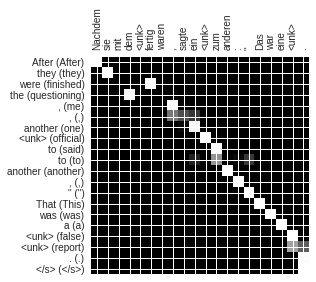
\includegraphics[width=.3\textwidth]{hw3/writeup/img/attn_vis_1.png}
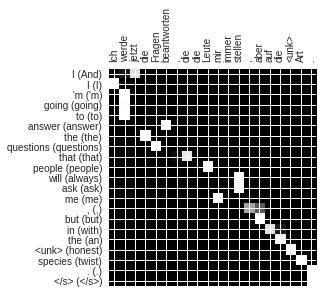
\includegraphics[width=.3\textwidth]{hw3/writeup/img/attn_vis_2.png}
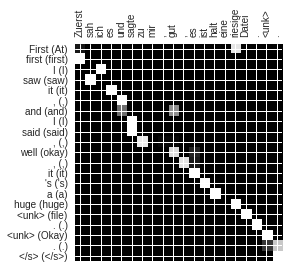
\includegraphics[width=.3\textwidth]{hw3/writeup/img/attn_vis_3.png}

\medskip

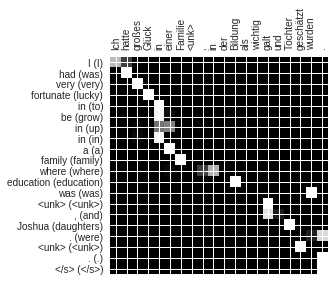
\includegraphics[width=.3\textwidth]{hw3/writeup/img/attn_vis_4.png}
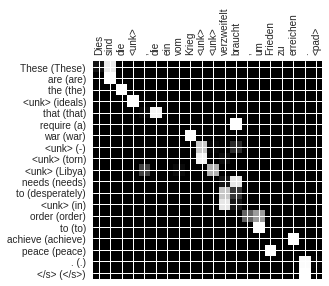
\includegraphics[width=.3\textwidth]{hw3/writeup/img/attn_vis_5.png}
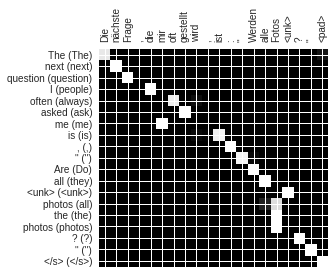
\includegraphics[width=.3\textwidth]{hw3/writeup/img/attn_vis_6.png}

\caption{Example sentence attention distributions. Lighter squares denote higher weights. The x-axis and y-axis of each plot correspond to words in the source sentence (German) and the generated translation (English) respectively. Along the y-axis for each plot, words in the parentheses are the true word, next to the model-predicted words.}
\label{pics:blablabla}
\end{figure}

Alignment regarding our source sentence and generated translations can then be characterized between individual words. Each row of a matrix indicates the weights associated with an annotation, and we are able to determine which positions in the source sentence were considered most important while generating the target word.

We note that the lighter diagonal paths across all our sample sentences suggests that our model pays attention to words in the source sentence in chronological order while decoding the target sentence, but there do seem to be a number of non-monotonic alignments. This seems reasonable when comparing two relatively similar languages such as English and German, which are both West Germanic languages. Accordingly, we suspect that these translations may empirically serve as a lower bound or baseline between neural machine translation tasks.



% For all models, we trained with $30$ epochs on batches of size $30$ unless otherwise noted. In addition to the Stanford SST-2 dataset supplied by torchtext, we implement all models as "named" versions using NamedTensor. As noted on Kaggle, we compare our submissions both with each other and a single class baseline, which achieves a public dataset testing accuracy of 52.38\%. Our basic results  are listed in Table 1.

% \begin{table}[h]
% \centering
% \begin{tabular}{llr}
%  \toprule
%  Model &  & Accuracy $(\%)$ \\
%  \midrule
%  \textsc{Single Class} & & 52.38\\
%  \textsc{Naive Bayes} & & 82.15 \\
%  \textsc{Logistic Regression} & & 78.41  \\
%  \textsc{CBOW} & &77.05 \\
%  \textsc{CNN} & & 79.49\\
%  \bottomrule
% \end{tabular}
% \caption{\label{tab:results} Basic model performance}
% \end{table}

% Although not actually implemented, we note that the single class baseline model does not perform well, with all other models exhibiting notable performance gains. Notably, although we did not expect Naive Bayes to be the top performer given its strong assumptions on input independence, our results show otherwise. 

% Given the successful performance of CNNs in \citet{DBLP:journals/corr/Kim14f}, we were interested in experimenting with the parameters and extending the models further. Our main objective was to try to reproduce the 87.2 \% accuracy reported on the SST-2 dataset. Accordingly, using default training parameters (filter lengths $2, 3, 4$; number of filters $100$ learning rate $2e^{-4}$; batch size $10$; dropout $0.5$), we experimented with stride length, filter lengths, hidden layer depth, and an alternate pre-trained embedding (GloVe). However, our results (summarized in Table 2) do not show clear improvements.

% \begin{table}[h]
% \centering
% \begin{tabular}{llr}
%  \toprule
% Model Modification &  & Accuracy $(\%)$ \\
%  \midrule
%  \textsc{Baseline} & & 79.49\\
%  \textsc{Stride Length} & & 80.07 \\
%  \textsc{Filter Lengths} & & 78.41  \\
%  \textsc{Embedding} & &81.49 \\
%  \bottomrule
% \end{tabular}
% \caption{\label{tab:results} Modified CNN model performance. \textbf{Stride Length}: Modification to the stride length from default length $1$, with optimal performance at length $2$. \textbf{Filter Lengths}: Adding a filter with size $2$ to the default filters of size $3, 4, 5$. \textbf{Embedding}: Building the vocab representation with Stanford's GloVe embedding}.
% \end{table}


% Finally we end with the experimental section. Each assignment will make clear the main experiments and baselines that you should run. For these experiments you should present a main results table. Here we give a sample Table~\ref{tab:results}. In addition to these results you should describe in words what the table shows and the relative performance of the models.

% Besides the main results we will also ask you to present other results
% comparing particular aspects of the models. For instance, for word
% embedding experiments, we may ask you to show a chart of the projected
% word vectors. This experiment will lead to something like
% Figure~\ref{fig:clusters}. This should also be described within the
% body of the text itself.

% \begin{figure}
%   \centering
%   \includegraphics[width=6cm]{cluster_viz}
%   \caption{\label{fig:clusters} Sample qualitative chart.}
% \end{figure}


\section{Conclusion}
We build, tuned, and trained different models to perform neural machine translation, with observed success compared to the baseline. Comparing the standard Seq2Seq model and a variant incorporating attention, we note note the improved performance in perplexity, consistent with the previous literature. Local attention thus empirically proves to be a source of boosted performance, observed with very few distinct modifications to the overall architecture of a standard encoder-decoder network. Although not implemented in our assignment, several state of the art methods employing more drastic changes to model architecture but relying on attention serve as promising future avenues of investigation.

% We built and trained different models to classify the SST data set, with overall success compared to the baseline. Surprisingly, the most successful model was Naive Bayes, which strongly assumes that features are independent of each other within a class. This may indicate that, in this data set, features more strongly correlated with a class actually tend to occur more independently of each other.

% Nevertheless, all of our models performed quite well. Although we were not able to replicate the CNN performance exhibited in \citet{DBLP:journals/corr/Kim14f}, we reached similar conclusions that with little hyperparameter tuning, a simple CNN with one layer of convolution and pre-trained embeddings worked well. In fact, the rather close performance of all model classes dependent on the our embedding, and the performance boost in CNNs seen when switching from the default wiki-based vectors to GloVe, further corroborate the idea that advances in NLP can be associated with unsupervised pretraining of word vectors. 


% The biggest difficulty we had throughout this process was acquainting ourselves with NamedTensor and sorting out bugs in our code resulting from the new package.  As a whole, we found the use of named dimensions to be very useful, but had to spend a bit more time wrangling and managing our data.\\


Our code can be found at \url{https://github.com/rpadaki/cs287assignments/tree/master/hw3}.

\bibliographystyle{apalike}
\bibliography{writeup}

\end{document}

